
Evaluating the performance of a poker player is a challenging task. Unfortunately, the majority of strong AI poker players are not publicly available. Furthermore, conducting a big-scale experiment against human players is also not feasible, as the big online poker-playing sites prohibit the use of bots. To get an idea of the performance of PokerShark, we conducted a number of experiments where PokerShark played against dummy-AI player and human players. To study the effect of the risk attitude on the agent's behavior, we repeated the experiments where PokerShark played against dummy-AI players using different risk attitudes.

In this section, the graphs are used to demonstrate how PokerShark's winnings changed throughout the games. For each opponent, the graphs display three lines: the red line represents the number of chips won before the showdown (i.e., when one of the players has folded), the blue line shows the winnings only at the showdown, and the green line is the cumulative total of PokerShark's winnings. The y-axis of each graph shows the number of chips, and the x-axis represents the round number.

Another important metric we use to evaluate the performance of PokerShark is WPH, which represents the average amount a player wins in each game round measured in small blinds. It is calculated by dividing the total winnings by the number of rounds played times the small blind amount. For example, if the agent always folds, it would have a WPH of -1,5 small blinds per round.

\section{Dynamic Risk Attitude}
For the experiments in this section, we used the dynamic attitude discussed in section 3.3.1 and the corresponding utility functions discussed in section 3.4.7. To summarize the ideas discussed in the previously mentioned sections, PokerShark adopts a risk-neutral attitude most of the time. The agent changes its attitude toward risk as the number of chips in its stack changes. When the stack of chips starts getting smaller, the agent changes its risk attitude to be more risk-averse. If the stack becomes significantly bigger than the starting amount, then the agent adopts a more risk-seeking attitude.

\subsection*{Playing against Dummy-AI players}
Dummy-AI players are AI players that use a simple static strategy to play poker. We used four such players: Bold, Fish, Honest and Random. The bold player always raises the maximum allowed amount regardless of his pocket. Similarly, the fish player always calls, whereas the honest player chooses the best action based on the estimated strength of his hand; finally, the random player chooses a random action.
At first glance, one might overlook the challenges imposed by these simple strategies. However, playing against these bots will provide a good chance to see how PokerShark will identify and exploit the weaknesses of each bot.


\subsubsection{Bold Player}
The bold player imposes an interesting problem because the bot will start each round by betting the entire stack; calling such a bet is very risky from the preflop. Looking at the graph shown in figure \ref{fig:results_bold}, we can see that most losses occur before the showdown because PokerShark is folding many weak hands. Although it is a very difficult challenge, PokerShark lost only 0.71 small blinds per hand. This is a very good result, considering that the bold player is a very loose and aggressive player.

\begin{figure}[H]
    \centering
    \begin{minipage}{\textwidth}
        \begin{minipage}{0.40\textwidth}
            \begin{tabular}{|l|l|l|}
                \hline
                \textbf{Number of games}  & 100   &        \\ \hline
                \textbf{Games won}        & 38    & 38.0\% \\ \hline
                \textbf{Games drew}       & 0     & 00.0\%  \\ \hline
                \textbf{Games lost}       & 62    & 62.0\% \\ \hline
                \textbf{Number of rounds} & 3237  &        \\ \hline
                \textbf{Rounds won}       & 110   & 30.4\%  \\ \hline
                \textbf{Rounds drew}      & 0     & 00.0\%  \\ \hline
                \textbf{Rounds lost}      & 3127  & 96.6\% \\ \hline
                \textbf{WPH}              & -0.71 &        \\ \hline
            \end{tabular}
        \end{minipage}
        \hspace{0.05\textwidth}
        \begin{minipage}{0.5\textwidth}
            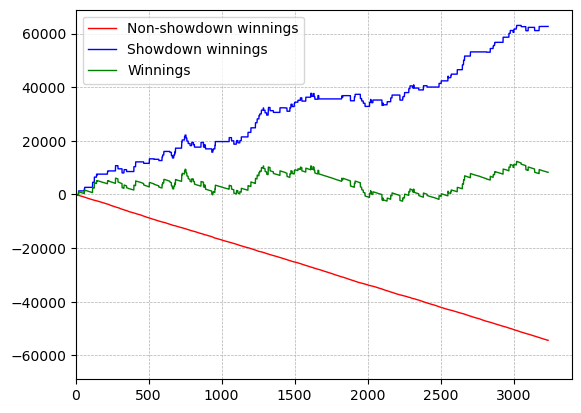
\includegraphics[width=\textwidth]{graphics/bold.png}
        \end{minipage}
    \end{minipage}
    \caption{Results of playing 100 games against the Bold player.}
    \label{fig:results_bold}
\end{figure}

\subsubsection{Fish Player}
Playing against the fish player is a good opportunity to showcase PokerShark's ability to exploit players' tendencies. For example, we can see from the Non-showdown winnings in figure \ref{fig:results_fish} that PokerShark did not fold as much, meaning it has adjusted its folding range. We can also see that although PokerShark is calling/raising a lot more, it manages the risk by using small raises.

\begin{figure}[H]
    \centering
    \begin{minipage}{\textwidth}
        \begin{minipage}{0.40\textwidth}
            \begin{tabular}{|l|l|l|}
                \hline
                \textbf{Number of games}  & 100  &        \\ \hline
                \textbf{Games won}        & 68   & 68.0\% \\ \hline
                \textbf{Games drew}       & 0    & 00.0\%  \\ \hline
                \textbf{Games lost}       & 32   & 32.0\% \\ \hline
                \textbf{Number of rounds} & 3385 &        \\ \hline
                \textbf{Rounds won}       & 1511 & 44.6\% \\ \hline
                \textbf{Rounds drew}      & 21   & 00.6\%  \\ \hline
                \textbf{Rounds lost}      & 1853 & 54.7\% \\ \hline
                \textbf{WPH}              & 1.10 &        \\ \hline
            \end{tabular}
        \end{minipage}
        \hspace{0.05\textwidth}
        \begin{minipage}{0.5\textwidth}
            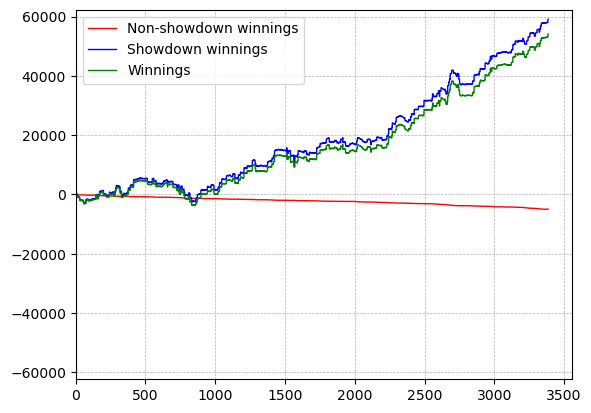
\includegraphics[width=\textwidth]{graphics/fish.png}
        \end{minipage}
    \end{minipage}
    \caption{Results of playing 100 games against the Fish player.}
    \label{fig:results_fish}
\end{figure}


\subsubsection{Honest Player}
Playing against a player that does not bluff is quite difficult because it folds when his hand is weak, and he only raises with a strong hand. Therefore, knowing when to challenge such a player is crucial to winning the game. Looking at the figure \ref{fig:results_honest}, we can see the games were more dynamic, with PokerShark successfully winning big bets but also lost many small bets with varying tolerance to call the raises of the honest player. Overall, We think PokerShark performed well against this player.
\begin{figure}[H]
    \centering
    \begin{minipage}{\textwidth}
        \begin{minipage}{0.40\textwidth}
            \begin{tabular}{|l|l|l|}
                \hline
                \textbf{Number of games}  & 100   &        \\ \hline
                \textbf{Games won}        & 17    & 17.0\% \\ \hline
                \textbf{Games drew}       & 0     & 00.0\%  \\ \hline
                \textbf{Games lost}       & 83    & 83.0\% \\ \hline
                \textbf{Number of rounds} & 9340  &        \\ \hline
                \textbf{Rounds won}       & 3670  & 39.3\% \\ \hline
                \textbf{Rounds drew}      & 3     & 00.6\%  \\ \hline
                \textbf{Rounds lost}      & 5667  & 60.7\% \\ \hline
                \textbf{WPH}              & -0.16 &        \\ \hline
            \end{tabular}
        \end{minipage}
        \hspace{0.05\textwidth}
        \begin{minipage}{0.5\textwidth}
            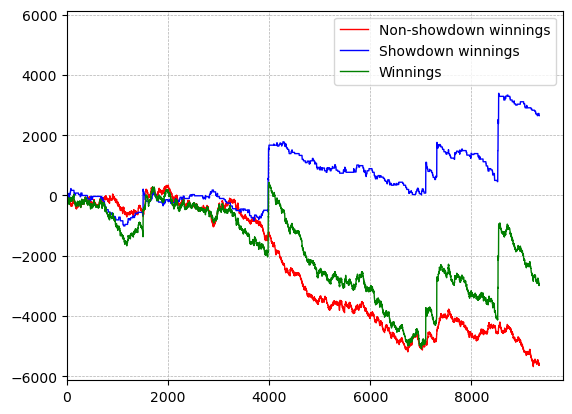
\includegraphics[width=\textwidth]{graphics/honest.png}
        \end{minipage}
    \end{minipage}
    \caption{Results of playing 100 games against the Honest player.}
    \label{fig:results_honest}
\end{figure}


\subsubsection{Random Player}
Facing a random opponent is a great way to see how PokerShark handles contradictory information while modeling its opponent. The graph in figure \ref{fig:results_random} shows how PokerShark used bigger betting amounts while also folding more often. 

\begin{figure}[H]
    \centering
    \begin{minipage}{\textwidth}
        \begin{minipage}{0.40\textwidth}
            \begin{tabular}{|l|l|l|}
                \hline
                \textbf{Number of games}  & 100   &        \\ \hline
                \textbf{Games won}        & 48    & 48.0\% \\ \hline
                \textbf{Games drew}       & 0     & 00.0\%  \\ \hline
                \textbf{Games lost}       & 52    & 52.0\% \\ \hline
                \textbf{Number of rounds} & 4540  &        \\ \hline
                \textbf{Rounds won}       & 1276  & 28.1\% \\ \hline
                \textbf{Rounds drew}      & 0     & 00.6\%  \\ \hline
                \textbf{Rounds lost}      & 3264  & 71.9\% \\ \hline
                \textbf{WPH}              & -0.03  &        \\ \hline
            \end{tabular}
        \end{minipage}
        \hspace{0.05\textwidth}
        \begin{minipage}{0.5\textwidth}
            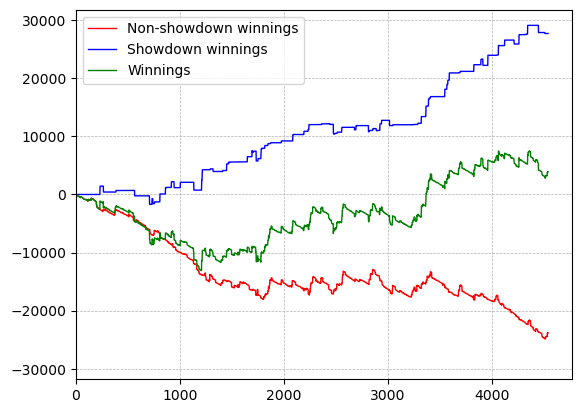
\includegraphics[width=\textwidth]{graphics/random.png}
        \end{minipage}
    \end{minipage}
    \caption{Results of playing 100 games against the Random player.}
    \label{fig:results_random}
\end{figure}

\subsection{Playing against human players}
Unfortunately, we could not organize a big experiment to test PokerShark's performance against human players. However, we were able to organize a few games with novice poker players. In total, PokerShark played a round thousand hands against human players.

\begin{figure}[H]
    \centering
    \begin{minipage}{\textwidth}
        \begin{minipage}{0.40\textwidth}
            \begin{tabular}{|l|l|l|}
                \hline
                \textbf{Number of games}  & 18   &        \\ \hline
                \textbf{Games won}        & 10    & 55.6\% \\ \hline
                \textbf{Games drew}       & 0     & 00.0\%  \\ \hline
                \textbf{Games lost}       & 8    & 44.4\% \\ \hline
                \textbf{Number of rounds} & 955  &        \\ \hline
                \textbf{Rounds won}       & 359  & 37.6\% \\ \hline
                \textbf{Rounds drew}      & 1     & 00.1\%  \\ \hline
                \textbf{Rounds lost}      & 595  & 62.3\% \\ \hline
                \textbf{WPH}              & 0.19  &        \\ \hline
            \end{tabular}
        \end{minipage}
        \hspace{0.05\textwidth}
        \begin{minipage}{0.5\textwidth}
            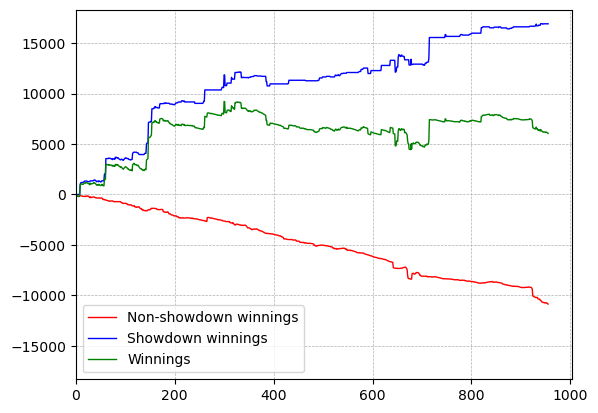
\includegraphics[width=\textwidth]{graphics/human.png}
        \end{minipage}
    \end{minipage}
    \caption{Results of around 1000 hands against human players.}
    \label{fig:results_human}
\end{figure}

Observing the graph shown in figure \ref{fig:results_human}, it is clear that PokerShark forfeited a significant portion of its profits by folding. That is due to the majority of human players being able to quickly identify and exploit PokerShark's tendency to fold when calling is too risky. The big fluctuations in winnings indicate that PokerShark did not always fold but was also able to call the opponent's bluff and score big wins.

\pagebreak
\section{Static Risk Attitude}
To investigate the impact of risk attitude on an agent's behavior, we reconducted the previous experiments in which PokerShark played against dummy AI players but this time using static risk attitudes.

The first set of experiments was run with the risk attitude of PokerShark being set to risk-seeking. Having a more risk-seeking attitude can change the behavior of a poker player in several ways. For one, a player who is more willing to take risks will be more likely to bet or raise with weaker hands since they are more willing to gamble in order to potentially win a larger pot. This can make them more unpredictable and difficult for their opponents to read. Additionally, risk-seeking players may also be more likely to bluff since they are more willing to risk betting with a weak hand to try and scare their opponents. Overall, a risk-seeking attitude should make PokerShark more aggressive and less predictable in its betting and playing style.

The second set of experiments was conducted with PokerShark having a risk-averse attitude. Having a risk-averse attitude can change the behavior of the agent, causing it to be more conservative in its betting and playing style. This should make PokerShark less likely to take risks, such as going all-in on a hand or making large bets, in order to avoid the potential loss of chips. 

The last set of experiments was conducted using a risk-neutral attitude, which should make PokerShark play in a similar style to the Honest player. Only calling or raising when it thinks it has the strongest hand. The detailed analysis of the games conducted is provided in appendix \ref{appendix:experiments}. We have also summarized the findings in table \ref{table:staticRiskAttitude}.


\begin{table}[h]
    \centering
    \begin{tabular}{ll|l|l|l|l|}
    \cline{3-6}
                                                                           &                       & \textbf{Win} & \textbf{Drew} & \textbf{Lost} & \textbf{WPH} \\ \hline
    \multicolumn{1}{|c|}{\multirow{4}{*}{\textit{\textbf{Bold Player}}}}   & \textbf{Dynamic risk} &    38.0\%    &     0.0\%     &     62.0\%    &    -0.71     \\ \cline{2-6} 
    \multicolumn{1}{|c|}{}                                                 & \textbf{Risk seeking} &    44.0\%    &     0.0\%     &     56.0\%    &    -0.47     \\ \cline{2-6} 
    \multicolumn{1}{|c|}{}                                                 & \textbf{Risk averse}  &    49.0\%    &     0.0\%     &     51.0\%    &    -0.04     \\ \cline{2-6} 
    \multicolumn{1}{|c|}{}                                                 & \textbf{Risk neutral} &    40.0\%    &     0.0\%     &     60.0\%    &    -0.57     \\ \hline
    \multicolumn{1}{|l|}{\multirow{4}{*}{\textit{\textbf{Fish Player}}}}   & \textbf{Dynamic risk} &    68.0\%    &     0.0\%     &     32.0\%    &     1.10     \\ \cline{2-6} 
    \multicolumn{1}{|l|}{}                                                 & \textbf{Risk seeking} &    77.0\%    &     0.0\%     &     23.0\%    &     1.70     \\ \cline{2-6} 
    \multicolumn{1}{|l|}{}                                                 & \textbf{Risk averse}  &    74.0\%    &     0.0\%     &     26.0\%    &     1.20     \\ \cline{2-6} 
    \multicolumn{1}{|l|}{}                                                 & \textbf{Risk neutral} &    76.0\%    &     1.0\%     &     23.0\%    &     1.58     \\ \hline
    \multicolumn{1}{|l|}{\multirow{4}{*}{\textit{\textbf{Honest Player}}}} & \textbf{Dynamic risk} &    17.0\%    &     0.0\%     &     83.0\%    &    -0.16     \\ \cline{2-6} 
    \multicolumn{1}{|l|}{}                                                 & \textbf{Risk seeking} &    92.0\%    &     1.0\%     &     7.0\%     &     0.40     \\ \cline{2-6} 
    \multicolumn{1}{|l|}{}                                                 & \textbf{Risk averse}  &    13.0\%    &     0.0\%     &     87.0\%    &    -0.26     \\ \cline{2-6} 
    \multicolumn{1}{|l|}{}                                                 & \textbf{Risk neutral} &    16.0\%    &     0.0\%     &     84.0\%    &    -0.16     \\ \hline
    \multicolumn{1}{|l|}{\multirow{4}{*}{\textit{\textbf{Random Player}}}} & \textbf{Dynamic risk} &    48.0\%    &     0.0\%     &     52.0\%    &    -0.03     \\ \cline{2-6} 
    \multicolumn{1}{|l|}{}                                                 & \textbf{Risk seeking} &    55.0\%    &     0.0\%     &     45.0\%    &     0.39     \\ \cline{2-6} 
    \multicolumn{1}{|l|}{}                                                 & \textbf{Risk averse}  &    27.0\%    &     0.0\%     &     73.0\%    &    -0.67     \\ \cline{2-6} 
    \multicolumn{1}{|l|}{}                                                 & \textbf{Risk neutral} &    16.0\%    &     0.0\%     &     84.0\%    &     0.36     \\ \hline
    \end{tabular}
    \caption{Results of playing 100 games using the different static risk attitudes.}
    \label{table:staticRiskAttitude}
\end{table}

The different risk attitudes yielded varying results against different players. Overall, the dynamic attitude performed the worst on average, with risk-seeking outperforming all other attitudes. This could be due to the nature of the game, or perhaps the experiments we conducted favored this attitude. Table \ref{table:average} shows how each attitude performed on average.

\begin{table}[h]
    \centering
    \begin{tabular}{|l|l|}
    \hline
    \textbf{Attitude} & \textbf{WPH} \\ \hline
    Dynamic risk      & 0.05         \\ \hline
    Risk seeking      & 0.51         \\ \hline
    Risk averse       & 0.06         \\ \hline
    Risk neutral      & 0.30         \\ \hline
    \end{tabular}
    \caption{Average WPH for each risk attitude.}
    \label{table:average}
\end{table}



\section{Self Play Experiments}
Due to the findings of our earlier experiments, we have chosen to conduct additional self-play experiments in order to further investigate the effect of risk attitude on the performance of the agent. To evaluate the impact of different risk attitudes on performance more thoroughly, we set up a series of head-to-head games between multiple copies of PokerShark, each with a different risk attitude. We wanted to see how the different risk attitudes would affect the outcome of the games, so we had each copy play 100 games against each of the other copies. This was important to verify the findings of our previous experiments.

\begin{table}[h]
    \centering
\begin{tabular}{l|c|c|c|c|c|}
\cline{2-6}
                                            & \textbf{Dynamic} & \textbf{Risk-Seeking} & \textbf{Risk-Averse} & \textbf{Risk-Neutral} & \textbf{Average} \\ \hline
\multicolumn{1}{|l|}{\textbf{Dynamic}}      & -                & -0.33                 & 0.01                 & 0.02                  & \textbf{-0.10}   \\ \hline
\multicolumn{1}{|l|}{\textbf{Risk-Seeking}} & 0.33             & -                     & 0.37                 & 0.36                  & \textbf{0.35}    \\ \hline
\multicolumn{1}{|l|}{\textbf{Risk-Averse}}  & -0.01            & -0.37                 & -                    & -0.01                 & \textbf{-0.13}   \\ \hline
\multicolumn{1}{|l|}{\textbf{Risk-Neutral}} & -0.02            & -0.36                 & 0.01                 & -                     & \textbf{-0.12}   \\ \hline
\end{tabular}
\caption{Results of self play with different risk attitudes; WPH of player at start of row}
\label{table:selfPlay}
\end{table}

Table \ref{table:selfPlay} shows the results of WPH for the player at the start of the row against the player at the start of the column. The results clearly show that the risk-seeking attitude outperforms all other attitudes. The dynamic risk attitude performed better than all other attitudes, which contradicts our previous experiments. However, it aligns with our initial intuition.

A larger experiment with human players would be required to make confident conclusions about the impact of risk attitude on performance. However, for now, we are led to believe that the domain of poker tends to favor risk-seeking players.